\documentclass[10pt,a4paper]{article}
\usepackage{caratula}
\usepackage{geometry}
\renewcommand\familydefault{\sfdefault} % Default family: serif 
\usepackage[usenames,dvipsnames]{xcolor}
\usepackage{tikz}
\usepackage{soul}
\usetikzlibrary{calc} 
\usetikzlibrary{arrows, decorations.markings,positioning,backgrounds,shapes}
\definecolor{EMP}{HTML}{77DD77} % Green1
\definecolor{NOR}{HTML}{06500C} % Green2
\usepackage{ulem}
\renewcommand{\ULdepth}{3pt}
\usepackage{tikz-dependency}
\usepackage{graphicx} 
\usepackage{indentfirst}
\setlength{\parindent}{12pt}

%\usetikzlibrary{positioning}




\titulo{TP1 }
\subtitulo{Relación PBI - Cantidad de sedes Argentinas en el exterior}

\fecha{\today}

\materia{Laboratorio de Datos}
\grupo{GRUPO 100}

\integrante{Chapana Puma, Joselin Miriam}{1197/21}{yoselin.chapana@gmail.com}
\integrante{Martinelli, Lorenzo}{364/23}{martinelli.lorenzo12@gmail.com}
\integrante{Padilla, Ramiro Martin}{1636/21}{ramiromdq123@gmail.com}

\graphicspath{{../static/}}


\begin{document}
\newgeometry{margin=2cm}

\maketitle

\restoregeometry
%\newgeometry{top=3cm,bottom=3cm,right=3cm,left=3cm} para editar margenes menos del titulo 


\section{Resumen} \vspace{0.3cm}

Estuve pensando y aca podriamos contar que fuimos pensando a lo largo del trabajo, los problemas con los que nos encontramos y como fue la dinámica, mas que nada porque la explicacion de la metodologia a seguir está en la parte de introducción.

\section{Introducción} \vspace{0.1cm}

\subsection{Objetivo y Fuente} \vspace{0.3cm}

El objetivo principal de este trabajo es encontrar una relación entre la cantidad de sedes de Argentina en un país y su PBI, si este será mayor, menor o si influirá la cantidad de secciones que una sede posea.  Para esto, trabajaremos con los siguientes datos, 

\begin{itemize}
	\item PBI per cápita de los paises (1)
	\item Representaciones Argentinas en el exterior, donde tenemos, Datos básicos de las sedes, Datos completos de sedes y secciones (2)
\end{itemize}

\noindent (1) Extraido de la pagina del Banco Mundial, https://data.worldbank.org/indicator/NY.GDP.PCAP.CD \\

\noindent (2) Obtenidas del Ministerio de Relaciones Exteriores, Comercio Internacional y Culto, \\ https://datos.gob.ar/dataset/exterior-representaciones-argentinas \vspace{0.1cm}
 
\subsection{Procedimiento} \vspace{0.3cm}

\indent Este trabajo tendrá varias etapas, comenzando con el planteo de un Diagrama de Entidad Relacional (DER) adecuado al objetivo de nuestro trabajo, es decir, a partir de los datasets mencionados anteriormente, nos quedaremos solo con aquellos datos necesarios para resolver nuestro problema. Luego, pasaremos nuestro DER al modelo relacional, el cual se encontrará en tercera forma normal y especificará claves primarias (PK), claves candidatas (CK), claves foráneas (FK) y dependencias funcionales. \par
Una vez tengamos nuestro modelo planteado, pasaremos a Python donde realizaremos una limpieza de los datos tomando ciertas decisiones que estarán explicadas hacia el final de este informe. 
Finalmente, con los datos ya limpios, a traves de distintas librerias como Pandas, Matplotlib, Inlinesql, entre otras nos encargaremos de consultar, manipular y visualizar los datos necesarios para dar con nuestro objetivo.


\newpage

\section{Procesamiento de Datos} \vspace{0.2cm}

Antes de comenzar con el procesamiento de datos, nos encontramos con las fuentes de datos originales en distintas formas normales. Comenzando con lista-sedes-datos y lista-secciones tenemos que ninguna de ambas se encuentra en primera forma normal puesto que el atributo redes-sociales de la primera y, el atributo telefonos\_principales de la segunda tenian valores no atómicos. Al no estar, en 1FN 
tampoco se encontraran en 2FN. \par
Por otro lado, la tabla que contiene el pbi de los paises, está en primera y segunda forma normal, sin embargo no se encuentra en tercera forma normal puesto que tiene dependencias transitivas, en particular, de Indicator Code $\rightarrow$ Indicator Name. \par
Y, por último, la tabla con la lista de sedes básica (la cual no utilizamos), está en segunda forma normal, pero no está en tercera forma normal puesto que tiene dependencias transitivas como por ejemplo, pais\_iso\_3 $\rightarrow$ pais\_iso\_2, considerenado clave primaria
a sede\_id.

\subsection{Limpieza de Datos}

Buscando mejorar la calidad de datos, encontramos problemas de instancia, por ejemplo, datos inconsistentes, problemas de 
procesos, puesto que hay diferentes criterios en la carga de los datos. Ahora, veamos cada dataset en detalle,

\begin{enumerate}
	\item lista-sede-datos, en ella, encontramos un problema asociado a instancia en el atributo 'redes\_sociales' que influye en su consistencia puesto que no hay un criterio unificado a la hora de cargar redes sociales. Por ejemplo, tenemos datos cargados en forma de URL donde es facil identificar a que red social pertenece, y por otro lado, tenemos datos que contienen, intuimos, nombres de usuarios, pero
no podemos discernir su red social. Para tener una medida concreta acerca de la magnitud del problema utilizamos el método GQM de la siguiente manera:
\begin{itemize}
	\item Goal : Evitar que haya datos que no se puedan identificar con alguna red social.
	\item Question : ¿Cual es la cantidad de elementos en redes\_sociales que no podemos identificar?
	\item Metrica :  Proporcion de registros sin campo redes\_sociales que son Urls o comienzan con @.  (0.23)
\end{itemize}
Para corregir esta tabla, además, seleccionamos columnas que consideramos relevantes para la resolución de nuestro problema principal. Puesto que teniamos datos redundantes, como dos codigos para un mismo pais o su traducción al inglés. También, consideramos mantener unicamente los datos de redes sociales que eran consistentes, es decir, eran Urls o comenzaban con @.
	\item En tabla correspondiente al PBI, API\_NY.GDP.PCAP.CD\_DS2\_en\_csv\_v2\_73.csv, tenemos también un problema de instancia, que afecta en particular, la completitud del atributo '2022'. Asi como también, otro problema de instancia es que encontramos muchos datos que no corresponden a paises. Estos fueron limpiados antes de elaborar la siguiente métrica,
\begin{itemize}
	\item Goal : Tener el dato '2022' quie refiere al Pbi de cada país completo,.
	\item Question : ¿Es relevante la proporcion de paises con el dato '2022' vacio?
	\item Metric: Proporcion de paises con el campo '2022' vacio. (0.09)
\end{itemize}
Para corregir este dataset, en primeria instancia, descartamos todas las columnas que no aportaban a nuestro objetivo, como por ejemplo, 
todas aquellas correspondientes a años anteriores a 2022. En segunda instancia, eliminamos aquellos datos que no correspondian con paises, 
por ejemplo 'Africa'. En último lugar, consideramos que al ser tan baja la proporcion de nulls, era conveniente descartarlos. 
	\item Por último, en lista-secciones, nos quedamos unicamente con las dos primeras columnas, sede\_id y descripción, en las cuales no encontramos ningun problema de calidad.
\end{enumerate}

\subsection{Diagrama de Entidad Relacional} \vspace{0.2cm}

Una vez planteado nuestro objetivo, nos encargamos de ver que datos necesitabamos para alcanzarlo, y como estarian representados. Para esto, elaboramos el siguien diagrama de entidad
relacional.  \vspace{0.2cm}

\begin{figure}[ht]
	\centering
	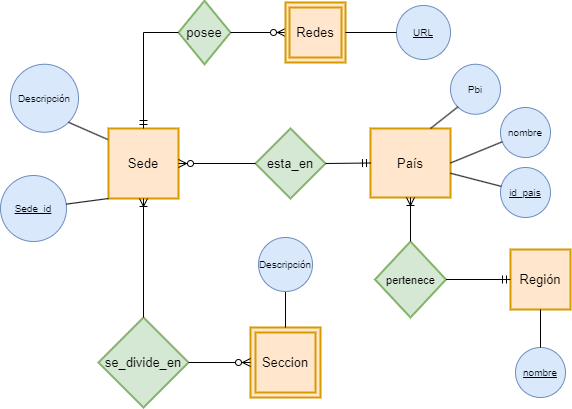
\includegraphics[width=1\textwidth]{DerFinal.png}
	\caption{Diagrama de Entidad Relacional}
	\label{fig:ejemplo}
\end{figure} \vspace{0.1cm}

Como se puede ver en la imagen anterior, consideramos que,

\begin{itemize}
	\item Una sede esta en un país y solo en uno.
	\item Un País puede tener muchas o ninguna sede.
	\item Las secciones existen pues existen las sedes, entonces, lo consideramos una entidad debil.
	\item Una sección puede estar en una o muchas Sedes, por ejemplo, la Embajada en Brasil y en Chile tiene su sección Administración.
	\item Una sede tiene al menos una sección.
	\item Cuando hablamos de Redes, hablamos mas de un perfil en una red social, por lo tanto, una red puede pertenecer a una y solo una sede.
\end{itemize}


\subsection{Modelo Relacional} \vspace{0.2cm}

Una vez que tenemos nuestro esquema gráfico, pasamos al planteo del modelo relacional. Notar que, las flechas representan las Foreign Keys y aquellos atributos 
subrayados representan las Primary Keys. En todas las relaciones, exceptuando a País, las Claves coinciden con las claves candidatas, esto se debe a que en País consideramos también a 
nombrePais como una posible clave.  \vspace{0.4cm}

\newbox\ubox

\begin{tikzpicture}[
    EMP/.style={% Style for empatized boxes
        rectangle, line width =1pt,
        anchor=west,
        underline, % new property
        align=center,
        text=Black,
        minimum height=.8cm,
        text height=1.7ex,
            text depth=.25ex,
        fill=EMP,
        draw=black,
        },
    NOR/.style={% Style for normal boxes.
        rectangle, 
        line width =1pt,
        anchor=west,
        align=left,
        minimum height=.6cm,
        text height=1.5ex,
            text depth=.25ex,
            text=white,
        fill=NOR,
        draw=black,
        inner ysep=5pt
        },
    underline/.append style={% define new style property
        execute at begin node={%
            \setbox\ubox=\hbox\bgroup
            },
            execute at end node={%
                \egroup\uline{\box\ubox}%
                }
             },
    ] % Uff that is all the configuration for tickzpicture xD

% Define an brute force objet "Frame"
% Variables 1:Position, 2: Identifier, 3: Title of frame 4: Subframe/Boxtype
 \def\Frame(#1)#2[#3]#4{%
  \begin{scope}[shift={(#1)}] 
      \node[font=\bf, anchor=west] (Title) at (-0.2,0.7) {#3}; 
       \edef\k{0}% Variable for box positión
       \edef\x{0}% Variable for named coordinate centering - below box
       \foreach \id/\style in {#4} {%enter sub frame data Name/Boxtype ,Name2/Boxtype | An space before Boxtype is needed 
            \node[\style] (h) at (\k pt,0) {\id}; %  % Draw a node depending on the variables.
            \pgfmathparse{\k+0.5*width{"\id"}+3.4pt} % Uses the textwidth to calculate named coordinate  
            \xdef\x{\pgfmathresult} % The resul is saved in the variable \x
            \draw (\x pt,-0.4) coordinate (\id#2); %Create a named coordinate concatenated: "sub frame data Name"+"identifier"
            \pgfmathparse{\k+width{"\id"}+6.8pt}% Calculate positión for each subframe box.       
        \xdef\k{\pgfmathresult}% Save the value to be added to the next iteration value.
       }    
  \end{scope}
}% disadvantages: Is not posible to use Frame data Name like: Name_another_desc instead I use Name-another-desc

% Start drawing
% \node[EMP node] (dm) at (0,0) {{Sometext/EMP,another/EMP}};
  \Frame(0,0){3}[PAIS]{
    IdPais/EMP,
    NombrePais/NOR,
    Pbi/NOR};

 \Frame(0,-2.5){1}[SEDE]{%first frame identified as 1 named EMPLOYEE
    IdSede/EMP,% see that it is necessary to add a space
    IdPais/NOR,
    Descripción/NOR}; 

 \Frame(0,-5){2}[REDES]{
    IdSede/EMP,
    Urls/EMP};  

 \Frame(0,-7.5){4}[REGION]{
    IdPais/EMP,
    Region/NOR};

  \Frame(0,-10){5}[SECCIONES]{
    IdSede/EMP,
    SeccionDescripcion/EMP};     

% Start drawing arrows:
% In this part I use the named coordinates to draw the arrows.
    \draw[thick,<-,thick,>=latex] % From Essn6 to Ssn1  
        (IdSede1)++(0.1,0) -- ++(0,-.55) -- ++(4.5,0) coordinate (inter) %inter is the name of coordinate register
        -- (IdSede2 -| inter) -- ++(0,-0.4) coordinate (inter)  % to calculate intersections.
        -- (IdSede2 |- inter) --++(0,0.4); %
        
    \draw[thick,<-,thick,>=latex]
        (IdPais3) -- ++(0,-.675) -- ++(5.2,0) coordinate (inter) 
        -- (IdPais4 -| inter) -- ++(0,-0.2) coordinate (inter) 
        -- (IdPais4 |- inter) --++(0,0.2); %

     \draw[thick,<-,thick,>=latex]
        (IdSede1)++(-0.3,0) -- ++(0,-.85) -- ++(4.3,0) coordinate (inter) 
        -- (IdSede5 -| inter) -- ++(0,-0.2) coordinate (inter) 
        -- (IdSede5|- inter) --++(0,0.2); %.
        
     \draw[thick,<-,thick,>=latex]
        (IdSede1)++(-0.3,0) -- ++(0,-.85) -- ++(4.3,0) coordinate (inter) 
        -- (IdSede5 -| inter) -- ++(0,-0.2) coordinate (inter) 
        -- (IdSede5|- inter) --++(0,0.2); %.

    \draw[thick,<-,thick,>=latex] % From Essn6 to Ssn1  
        (IdPais3)++(0.2,0) -- ++(0,-.5) -- ++(5.2,0) coordinate (inter) %inter is the name of coordinate register
        -- (IdPais1 -| inter) -- ++(0,-0.4) coordinate (inter)  % to calculate intersections.
        -- (IdPais1 |- inter) --++(0,0.45); %

 
\end{tikzpicture} \vspace{0.4cm}

Ahora, solo resta mostrar las dependencias funcionales de este modelo relacional para dejar en claro que se encuentra en la forma normal deseada (3FN) y, también tener completo nuestro esquema para asi comenzar a manipular los datos.

\newpage

\subsection{Dependencias Funcionales} \vspace{0.1cm}

A continuación, mostramos las dependencias funcionales de las relaciones de nuestro modelo relacional. En esta, se puede apreciar que 
todas se encuentran en segunda y tercera formal. Luego, con la limpieza de datos, garantizaremos que todos sus atributos sean atómicos
y por ende se encuentre también en primera forma normal.  \vspace{0.3cm}

\depstyle{lvl}{%
    edge height=2.5ex,
    % edge unit distance=#1*2.5ex, % Another way of controlling the appearance of the edges.
    edge below,
    edge horizontal padding=0,
    edge vertical padding=(#1-1)*3ex,
    text only label, % No need for label for functional dependencies.
    edge slant=0, % Right angles
    rounded corners=0,
    edge style={>=triangle 60} % Change the style of the arrowheads.
}
\tikzset{
    matrix/.append style={column sep=0.4cm} % Adding some distance between the attributes.
}
\tikzstyle{TxtBook}=[% Style to mimic the textbook Fundamentals of Database Systems.
    column sep=0cm, % No distance between two attributes.
    nodes={%
        fill=gray!20,
        draw=black,
        thick,
        inner xsep=3ex,
        inner ysep=1ex
    }
]
\tikzstyle{TxtBookChico}=[% Style to mimic the textbook Fundamentals of Database Systems.
    column sep=0cm, % No distance between two attributes.
    nodes={%
        fill=gray!20,
        draw=black,
        thick,
        inner xsep=1.2ex,
        inner ysep=1ex
    }
]


\textbf{Sede} \vspace{0.1cm}

\begin{dependency}
    \raggedright
    \begin{deptext}[TxtBookChico] % Applying the TxtBook style.
        \textbf{\underline{idSede}}  \& idPaís \& Descripción\\
    \end{deptext}
    \depedge[lvl=1]{1}{2}{}
    \depedge[lvl=1]{1}{3}{}
\end{dependency} \vspace{0.3cm}
 \vspace{0.3cm}

\textbf{País} 
\vspace{0.1cm}

\begin{dependency}
    \raggedright
    \begin{deptext}[TxtBook] % Applying the TxtBook style.
        \textbf{\underline{idPaís}}  \& NombrePaís \&Pbi \\
    \end{deptext}
    \depedge[lvl=1]{1}{2}{}
    \depedge[lvl=1]{1}{3}{}
    \depedge[lvl=2]{2}{1}{}
    \depedge[lvl=2]{2}{3}{}
\end{dependency} \vspace{0.3cm}

\textbf{Región} 
\vspace{0.1cm}

\begin{dependency}
    \raggedright
    \begin{deptext}[TxtBook] % Applying the TxtBook style.
        \textbf{\underline{idPaís}} \& Región  \\
    \end{deptext}
    \depedge[lvl=1]{1}{2}{}
\end{dependency} 

\vspace{3mm}
\textbf{Sección} 

\begin{dependency}
    \raggedright
    \begin{deptext}[TxtBook] % Applying the TxtBook style.
        \textbf{\underline{IdSede}}  \& \textbf{\underline{Sección}}  \\
    \end{deptext}
    \depedge[lvl=1]{1}{2}{}
    \depedge[lvl=1]{2}{1}{}
\end{dependency} \vspace{0.1cm}

Observación: la única DF es $\{$IdSede, Sección$\} \rightarrow \{$IdSede, Sección$\}$

\vspace{3mm}
\textbf{Redes} 

\begin{dependency}
    \raggedright
    \begin{deptext}[TxtBook] % Applying the TxtBook style.
        \textbf{\underline{IdSede}}  \& \textbf{\underline{redURL}}  \\
    \end{deptext}
	\depedge[lvl=1]{2}{1}{}
\end{dependency} \vspace{0.3cm}

\subsection{Importación de Datos} \vspace{0.3cm}

Una vez ya limpios los datos, creamos con pandas un archivo csv para cada relación de nuestro modelo. Luego, los importamos 
a los dataframe vacíos creados anteriormente.

\section{Decisiones tomadas}


\section{Análisis de datos}


\section{Conclusiones}

\end{document}